\def\stitle{\theexercise\ - Klassenhierarchien}
\section{\stitle}

\begin{frame}[fragile]%
  \frametitle{\stitle}%
Betrachten Sie die nachfolgenden Klassendefinitionen:

\begin{lstlisting}
public class Wal {};
public class Zahnwal extends Wal {};
public class Pottwal extends Zahnwal {};
public class Delphin extends Zahnwal {};
public class Bartenwal extends Wal {};
public class Grauwal extends Bartenwal {};
\end{lstlisting}

In der \code{main}-Methode eines Java-Programms findet man die Zeilen

\begin{lstlisting}
Wal w;
Zahnwahl z;
\end{lstlisting}

Entscheiden Sie, welche der folgenden Ausdr\"ucke g\"ultig sind.
\begin{center}
\begin{minipage}{0.49\textwidth}
\begin{enumerate}
\item \code{z = new Zahnwal();}
\item \code{z = new Delphin();}
\item \code{w = new Bartenwal();}
\item \code{z = new Bartenwal();}
\item \code{w = new Grauwal();}
\end{enumerate}
\end{minipage}
\begin{minipage}{0.49\textwidth}
\begin{enumerate}
\setcounter{enumi}{5}
\item \code{z = new Wal();}
\item \code{z = (Zahnwal) new Wal();}
\item \code{z = (Zahnwal) new Pottwal();}
\item \code{z = (Zahnwal) new Grauwal();}
\item \code{z = (Zahnwal) null;}
\end{enumerate}
\end{minipage}
\end{center}
\end{frame}


\begin{frame}[t]%
F\"ur die L\"osung dieser Aufgabe ist das folgende Klassendiagramm hilfreich.
Jeder Pfeil zeigt von einer Klasse auf deren Basisklasse.
\begin{center}
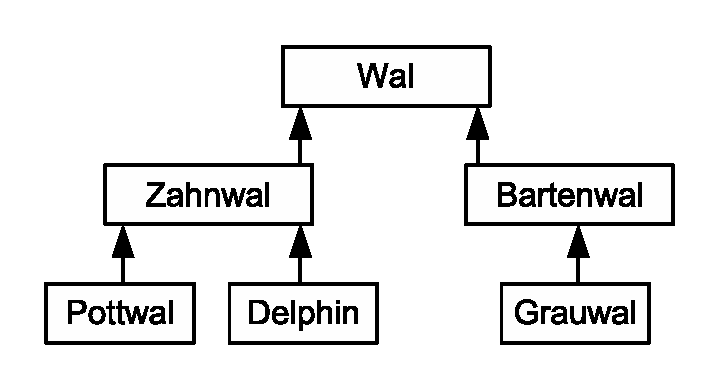
\includegraphics[height=4cm]{\getexercisefolder/wale}
\end{center}
\end{frame}

\begin{frame}[t]%

\begin{enumerate}
\item
  Der Ausdruck ist g\"ultig.
  Der Variable \code{z} vom Typ \code{Zahnwal} wird eine Instanz der Klasse \code{Zahnwal} zugewiesen.
\item
  Der Ausdruck ist g\"ultig.
  Die Klasse \code{Delphin} ist von der Klasse \code{Zahnwal} abgeleitet.
  Daher ist jede Instanz der Klasse \code{Delphin} auch eine Instanz der Klasse \code{Zahnwal} (\glqq Delphine sind Zahnwale.\grqq).
\item
  Der Ausdruck ist g\"ultig.
  Die Klasse \code{Bartenwal} ist von der Klasse \code{Wal} abgeleitet.
  Daher ist jede Instanz der Klasse \code{Bartenwal} auch eine Instanz der Klasse \code{Wal} (\glqq Bartenwale sind Wale.\grqq).
\item
  Der Ausdruck ist ung\"ultig.
  Die Klasse \code{Bartenwal} und die Klasse \code{Zahnwal} sind zwar beide von der Klasse \code{Wal} abgeleitet.
  Die Klasse \code{Bartenwal} ist jedoch nicht von der Klasse \code{Zahnwal} abgeleitet.
  Aus diesem Grund sind Instanzen der Klasse \code{Bartenwal} keine Instanzen der Klasse \code{Zahnwal} (\glqq Bartenwale sind keine Zahnwale.\grqq).
\item
  Der Ausdruck ist g\"ultig.
  Die Klasse \code{Grauwal} ist \"uber die Klasse \code{Bartenwal} von der Klasse \code{Wal} abgeleitet.
  Jede Instanz der Klasse \code{Grauwal} ist daher auch eine Instanz der Klasse \code{Wal} (\glqq Grauwale sind Wale.\grqq).
\end{enumerate}
\end{frame}

\begin{frame}[t]%

\begin{enumerate}
\setcounter{enumi}{5}
\item
  Der Ausdruck ist ung\"ultig.
  Die Klasse \code{Wal} ist Basisklasse der Klasse \code{Zahnwal}.
  Daher ist ein Instanz der Klasse \code{Wal} keine Instanz der Klasse \code{Zahnwal} (\glqq Nicht jeder Wal ist ein Zahnwal.\grqq).
\item
  Der Ausdruck ist ung\"ultig.
  Die Klasse \code{Wal} ist Basisklasse der Klasse \code{Zahnwal}.
  Die Typumwandlung von einer Basisklasse zu einer abgeleiteten Klasse ist nicht m\"oglich.
\item
  Der Ausdruck ist g\"ultig.
  Die Klasse \code{Pottwal} ist von der Klasse \code{Zahnwal} abgeleitet.
  Die Typumwandlung von einer abgeleiteten Klasse zur entsprechenden Basisklasse ist m\"oglich.
  Man beachte, dass die Typumwandlung auf die Instanz selbst keinen Einfluss hat, d.h{.} nach der Initialisierung ist in der Variable \code{z} eine Instanz der Klasse \code{Pottwal} gespeichert.
\item
  Der Ausdruck ist ung\"ultig.
  Die Klasse \code{Grauwal} ist nicht von der Klasse \code{Zahnwal} abgeleitet.
  Die Typumwandlung ist daher nicht m\"oglich.
\item
  Der Ausdruck ist g\"ultig. Die leere Referenz \code{null} verweist auf keine Instanz.
  Die Typumwandlung wird ohne jeden Effekt durchgef\"uhrt.
\end{enumerate}
\end{frame}
